\chapter{Introduction}
\graphicspath{{introduction/figs}}

\section{Tipping Points}
Take a pan of water and heat it up. As its temperature rises, some of the water's properties may change. For example, the viscosity and heat flux to the
environment may change. However, the water still remains as water and these changes will vary continuously with the water temperature. However, if the water is heated beyond
a critical temperature of \SI{100}{\degreeCelsius} something more dramatic happens and the water boils away. The properties of the resulting steam are quite different
to the original water --- a \emph{qualitative} change has occurred.

It is this sort of qualitative change that this thesis shall be concerned with. Whilst the boiling of water is a phase transition \parencite{Goldenfeld1992}, I shall use the broader terminology
of \emph{tipping points} \parencite{Lenton2008} or \emph{critical transitions} \parencite{Rahmstorf1995} or \emph{abrupt changes} \parencite{Alley2003} to describe these phenomena. I shall largely stick
to the term tipping point, or just tipping, which has its origins in the idea that when an object is lent over it will return to its original position unless it is lent over sufficiently far when the object
will tip over.

\subsection{Definitions}

Although it can be a vague term, the concept of a small nudge leading to a large change generally forms a part of most formal definitions of tipping points.
For example,~\cite{Lenton2008} defines the occurrence of a tipping
point as when a control parameter, there is a critical value $\rho_{\mathrm{crit}}$ of a control parameter, $\rho$, above which any significant variation, $\delta \rho > 0$ leads to a qualitative change
$\hat{F}$ of a system feature $F$, after some observation time $T > 0$. They write this mathematically as
\begin{equation}
  \label{eq:lenton_tipping_definition}
  |F(\rho \geq \rho_{\mathrm{crit}} + \delta \rho | T) - F(\rho|T)| \geq \hat{F} > 0.
\end{equation}
More recently,~\cite{ArmstrongMcKay2022} updated this definition by requiring $\delta \rho$ to be within the natural variability of the system. They also require that changes become self perpetuating
beyond $\rho_{\mathrm{crit}}$ as a result of the asymmetry of relevant feedbacks and that the tipping leads to `substantial' impacts. The IPCC \parencite{AR6} defines tipping differently still
as `a level of change in system properties beyond which a system reorganises, often in a nonlinear manner, and does not return to the initial state even if the drivers of the change are abated'.
Others, such as~\cite{Wang2023}, inspired by~\cite{Kopp2016}, insist that tipping points should occur on fast time scales.

Each of these definitions are deficient in their own way. The IPCC definition allows for linear behaviour, although tipping is a fundamentally nonlinear phenomenon. It also insists on \emph{hysteresis},
which is the property that the system does not return to its initial state after abating the drivers, although not all examples of tipping --- including boiling water --- experience this.
The complex definition in~\cite{Lenton2008} views tipping in terms of changes in parameters of a system, and not something a system can do spontaneously, which excludes certain types of
tipping (see \cref{sec:tipping_typology}). The third definition, that of~\cite{ArmstrongMcKay2022}, suffers from the problems of~\cite{Lenton2008} and also requires `substantial' impacts, which
artificially restricts the abrupt shifts that can be investigated. Finally,the requirement of~\cite{Wang2023} that tipping points be realised quickly is problematic for Earth System investigations
as some of the tipping points of interest will be realised slowly.

In this thesis, I will use the term tipping point in the sense that a system undergoes a tipping point when it experiences a qualitative change in its properties. Although this is a vague definition,
it enables the term tipping point to include all dynamics of interest. I am adopting Potter Stewart's philosophy that although a tipping point might be hard to define,
`I know it when I see it' \parencite{Stewart1964}.

\subsection{Examples of Tipping}

These sorts of nonlinear changes have long fascinated scientists. Physicists have investigated phase changes not just in terms of the boiling and freezing of substances but also
in magnetic materials \parencite{Ising1925,Onsager1944}, superconductivity \parencite{Landau1965} and percolation theory \parencite{Flory1941}. Each of these are different processes, but it is a
remarkable fact that near the phase transition different systems can be dynamically very similar, a phenomenon known as universality \parencite{Wilson1983}. This sort of idea --- that different examples
of tipping points across totally different systems can share many common features as been an important driving force in the theory of tipping points. 

Tipping points are also important in biology. In medicine, tipping point theory has been used to help understand asthma attacks \parencite{Donovan2022} and sleeping dynamics \parencite{Skeldon2014}.
Tipping points have proven very important in ecology. In an influential article, \parencite{May1976}, the ecologist Robert May noted that even very simple nonlinear models have rich dynamics and are capable
of experiencing tipping points (although he did use that term).~\cite{Holling1973} introduced the idea of resilience which is to do with the ability of a system to resist tipping. Tipping points have
been found in a range of ecosystems \parencite{Scheffer2001,Dakos2019}. The transition to turbid state in lakes \parencite{Scheffer1993} and the collapse of plant-pollinator communities
\parencite{Lever2014} are both examples of ecological tipping points, however other studies \parencite{Hillebrand2020} have challenged this.

Notions of multiple equilibria and the ability to transition between them has been used to explain patterns seen in nature. This was introduced by Turing \parencite{Turing1952} to explain
patterns found in certain plants and animals. Since then, it has been used to explain patterns in ecosystems \parencite{Rietkerk2008}.

\section{Tipping Points in the Earth System}
Whilst part of this thesis is applicable to many systems, the focus of this work has been on applications to the Earth system. In this section I want to give some background on these tipping
points, including outlining some mechanisms. I will focus on a few key sub subsystems. I will then discuss some of the evidence for tipping behaviour in the Earth's past.

The most recent IPCC report \parencite{AR6} finds it `unequivocal that human influence has warmed the atmosphere, ocean and land'. Humans have done this through the release of greenhouse
gases, most importantly carbon dioxide (\ce{CO2}), and also through land use change. This has led to observable changes in the Earths climate. Most obvious is the changes in global mean surface
temperature, with a most likely temperature increase of \SI{1.07}{\kelvin} \parencite{AR6} in the global mean but with clear regional differences \parencite{Morice2021} such as
Arctic amplification as well as more warming over land than over ocean. Other effects include rise of around \SI{0.2}{\meter} in sea levels \parencite{Frederikse2020} and increase in heavy precipitation
events \parencite{Fischer2016}.

\subsection{Tipping at the global scale}
This global warming is unprecedented in at least the last 2000 years and has caused global temperature levels not seen in the last $125,000$ years \parencite{AR6}. This naturally leads to a question
about the nature of the change the Earth system is experiencing: will it be a smooth function of increasing \ce{CO2} or is tipping behaviour possible?

A controversial paper,~\cite{Steffen2018}, considered the possibility that ongoing global warming could make the Earth transition from its current current glacial-interglacial limit cycle
state into a new `hothouse' state. This state would be defined by high temperatures and sea levels, posing challenges both to humanity and the wider biosphere. This state would be reached
through biogeochemical feedbacks leading to a cascade of tipping points. This would require humanity to operate with certain `planetary boundaries' \parencite{Rockstrom2009} to avoid this possibility.

Part of the reason~\cite{Steffen2018} proved so controversial is that there is little evidence this nonlinear response at the global scale. Global temperature rise is approximately linear
in emitted carbon dioxide \parencite{Allen2009,Rogelj2019} and not expected to continue after emissions cease \parencite{MacDougall2020}. However certain cloud resolving models
report that at sufficiently high levels of global warming stratocumulus cloud decks can break up causing \SI{8}{\kelvin} of warming globally \parencite{Schneider2019}.

\subsection{Tipping Elements}

However there is still the possibility of more regional tipping point behaviour. A foundational paper,~\cite{Lenton2008}, introduced the notion of \emph{tipping elements} which
are components of the Earth system that are `at least subcontinental in scale' ($\mathcal{O}(\SI{1000}{\kilo\meter}$) which can undergo tipping behaviour as a result of
anthropogenic influence. Lenton lead an expert elicitation of potential tipping elements in the Earth system to estimate how much warming would be needed to trigger the tipping element
and what the key uncertainties were. More recently,~\cite{ArmstrongMcKay2022} updated this study by reviewing the literature published since.  Following this, I will discuss some key tipping elements.

\subsubsection{Atlantic Meridional Overturning Circulation}
The Atlantic Meridional Overturning Circulation, known as the AMOC, is a large scale current in the ocean. The AMOC transports warm water polewards. This heat transport plays an
important role in the climate of, for example, northern Europe where it keeps temperatures warmer than they would be otherwise. The AMOC is driven by the salt-advection feedback, whereby
warm surface water is transported northwards where it cools and becomes more dense.  It then sinks and can make the return journey to the equator completing the circulation  \parencite{Vallis}.

The potential for the AMOC to exhibit bistability was postulated by Stommel in a pioneering paper \parencite{STOMMEL1961}. He showed in a simple two box model that if the North Atlantic was
freshened then the salt-advection feedback means that meridional transport could shift to a different state. Later work \parencite{Rahmstorf1995,Hawkins2011} found multistability in
complex ocean models, when the north Atlantic was subject to a `hosing' experiment in which fresh water was added to the oceans. Other research has shown the AMOC is sensitive to the
rate of hosing \parencite{Alkhayuon2019} in a complex way \parencite{Lohmann2021} in that there is not one critical rate of hosing. By this is meant that there is no well defined critical
hosing rate but that increasing the rate will switch the rate from a dangerous one and back again. Should the AMOC tip, this would have serious impacts on British agriculture
\parencite{Ritchie2020a}, global climate \parencite{Jackson2015} and the carbon cycle \parencite{Bozbiyik2011}.


Increased arctic precipitation, melting of the Greenland icesheet and increases in surface temperatures all act to weaken the AMOC \parencite{ArmstrongMcKay2022}.
Over the past half century, there is evidence that the AMOC has weaken by around 15\% \parencite{Caesar2018} and might be the weakest in a millennium \parencite{Caesar2021}.
There is observational evidence of decreasing AMOC stability \parencite{Boers2021a,Michel2022}. Some CMIP5 models show AMOC tipping at low
levels of global warming \parencite{Drijfhout2015}, although most models show only a gradual decline in the AMOC, which is helps explain why~\cite{AR6} view AMOC shutdown as
being unlikely, although they view the modelled AMOCs as being unrealistically stable.~\cite{ArmstrongMcKay2022} estimate the AMOC's threshold to be at \SI{4}{\degreeCelsius},
with a range of \SIrange{1.4}{8}{\degreeCelsius}.

\subsubsection{Ice Sheets} 
Ice sheets, found in Greenland and Antarctica are believed to be able to tipping behaviour due to many feedback processes. The melt elevation feedback, which is when an ice sheet melts and
therefore loses hight, exposing its surface to warmer air, increasing the melt rate, is an important feedback \parencite{Levermann2016}. Another relevent feedback is the
marine ice sheet instability, which occurs when the grounding line of an ice sheet meets a reverse slope \parencite{Schoof2007}.

Complex ice sheet models of Antarctica \parencite{Garbe2020} show hysteresis when global temperatures are reduced. Tipping behaviour has also been observed in complex models
of Greenland \parencite{Robinson2012,VanBreedam2020,Noel2021}. There is evidence of destabalisation in Greenland \parencite{Boers2021} and~\cite{ArmstrongMcKay2022} estimate
the critical threshold to be at around \SI{1.5}{\degreeCelsius}. For Antartica they estimate a similar threshold for the West Antarctic Ice Sheet but a higher threshold
of around \SI{8.5}{\degreeCelsius} for the East Antartic Ice Sheet. In all these cases, the tipping dynamics are very slow, taking $\mathcal{O}(\SI{1000}{\year})$ to materialise.

\subsubsection{Amazon Rainforest}
The Amazon Rainforest is a vast store of carbon, containing around \SI{123}{\peta\gram\carbon} \parencite{Malhi2006}, and has for many years been a sink, albiet a weaking one,
of anthropogenic carbon \parencite{Brienen2015}. The vegetation exerts an important influence on its local climate.
By shading, evapotranspiration and alebdo effects the rainforest affects its own temperature \parencite{Baker2019}.
Furthermore, the forest recycles its own rainfall, which acts to increase the precipitation it experiences \parencite{Spracklen2012}. It is
these feedback processes that give the potential for tipping.

Early coupled climate-carbon models \parencite{Cox2000} showed strong decreases in carbon stored in the Amazon. This dieback \parencite{Cox2004}  from a forested to a savannah state was
caused by drying in the Amazon, where 25\% of precipitation reductions over the Amazon under elevated \ce{CO2} was caused by forest feedbacks \parencite{Betts2004}.
However, Amazon dieback was found to be sensitive to the parametrisation of land surface interactions and the control climate\parencite{Huntingford2004}. Since then,
some CMIP5 models \parencite{Drijfhout2015} showed signs of Amazon dieback and CMIP6 models show examples of regional Amazon dieback \parencite{Parry2022}.

Other anthropogenic factors can cause abrupt shifts in the Amazon. An example is shifting fire regimes. Fire in the Amazon is driven by humans \parencite{UNEP2002}.
Furthermore fires occur generally below a tree cover threshold \parencite{Wuyts2017} and fires tend to decrease the tree cover so that as fires become more common in the
Amazon due to global warming \parencite{Cochrane2009} there could be a shift to a low tree cover high fire frequency regime \parencite{Wuyts2022}, behaviour
which has been seen in Dynamic Global Vegetation Models (DGVMs) \parencite{Lasslop2016}. This can be viewed
as being caused by a percolation process \parencite{Schertzer2015,Cardoso2022}.

Percolation theory has been used to understand the increasing fragmentation of tropical forests \parencite{Taubert2018}. They argued that as deforestation reduces forest area,
this causes an increase in the number of forest fragments. Based on results from percolation theory \parencite{Stauffer1994} they found tropical forests were near to the critical point.
Other work \parencite{Boers2017} has also found that deforestation in the Amazon can cause tipping as reduced transpiration of water weakens the feedbacks on the South American Monsoon system. 

There is observational evidence to believe that the Amazon is bistable, and that it is heading towards a tipping point. There exists a range of mean annual precipitation
such that Amazon tree cover can either be high or low, which is evidence of bistability \parencite{Hirota2011,Staver2011}.  Furthermore, states with lower mean annual
precipitation appear to be less stable \parencite{Ciemer2019}. There is evidence of drying in Amazonia \parencite{Ritchie2022}, which is a driver of dieback. There is now reason to
believe the Amazon is a soure of carbon to the atmosphere \parencite{Gatti2021}. There is are also indications of a loss of resilience in the Amazon \parencite{Boulton2022} which is
evidence of an approaching tipping point.

\cite{ArmstrongMcKay2022} estimate Amazon dieback to occur at global warming levels of \SIrange{2}{6}{\kelvin} with a best estimate of \SI{3.5}{\kelvin} but could be lower when the impact
of deforestation is included. Furthermore, timescales involved in this tipping point ($\mathcal{O}(\SI{100}{\year})$) are timescales of a human life, and so make this a very policy relevent
tipping point.

\subsubsection{Other Tipping Elements}
The Atlantic Meridional Overturning Circulation, ice sheets in Greenland and Antarctica and the Amazon Rainforest are three of the most important tipping elements in the Earth
system. However there are other proposed tipping elements. For example, high latitude permafrost may be at risk \parencite{Lenton2012a}, however there is debate about wether this is
a true threshold or a more continuous change \parencite{ArmstrongMcKay2022}. Climate model simulations have suggested the possibility of hydrological tipping points
\parencite{Teufel2019} would imply an increased risk of fire.

Coral reefs can have tipping behaviour, as coral death occurs at certain temperature thresholds \parencite{Frieler2013}. The tipping point occurs at around \SI{1.5}{\kelvin} of global
warming, as a result coral reefs are at high risk of tipping.

\subsection{Tipping Cascades}
In recent years, a number of scientists have investigated the possibility of tipping cascades
\parencite{Steffen2018,Wunderling2023,Wunderling2021,Rocha2018,Lenton2013a,Kriegler2009,Klose2021}.
A tipping cascade refers to situation where one tipping element tips, causing anothe tipping element to tip. For example, loss of Greenland icesheets could increase
the probability of the AMOC tipping \parencite{Caesar2018,Rahmstorf2015}. However, other interactions between tipping elements might have a stabalising effect, For example,
loss of the west Antarctic ice sheet could stabalise the AMOC \parencite{Sinet2023} due an increased meltwater flux.

Whilst much findings about tipping points are uncertain,
this is particularly acute in the case of research into tipping cascades where much of the research involves the use of conceptual models with highly stylised interactions between elements.
However, although many researchers would  regard these tipping elements and tipping cascades as unlikely to be triggered, they are often considered `too risky to bet against' \parencite{Lenton2019a}.
For instance,~\cite{Ritchie2020a} found that an AMOC collapse could end arable farming in Britain. The concept of being too risky to bet against relates to the fact
that catastrophic events dominate the costs in a cost benefit analysis \parencite{Weitzman2009} as long as they have a non-negligible probability of occuring.
To demonstrate that these events can occur, I will give some examples of abrupt shifts from the Earth's past.

\subsection{Evidence of Tipping Points from Paleoclimate}


\section{A Typology of Tipping Points}
\label{sec:tipping_typology}
\subsection{Bifurcation}
Poincare.
\subsubsection{Theory}
If $\dot{x} = f(x)$, show that $f'(x_{tip}) = 0$. Normal forms
\subsubsection{Stommel's AMOC Model}
\subsection{Noise}
\subsubsection{Theory}
Derive Kramers rate?
\begin{equation}
  \label{eq:kramers_law}
  \mathbb{E}(\tau) \sim \frac{2\pi}{\sqrt{V''(x_1)\left|V''(z)\right|}} \exp \left(\frac{V(x_1) - V(z)}{\sigma^2}\right)
\end{equation}
\subsubsection{D.O. Events}
\subsection{Rate}
\subsubsection{Theory}
3 diagrams unstable manifold
\subsubsection{Compost Bomb}
\subsection{Shock}
\subsubsection{Theory}
Calculate the distance to the boundary for a general fixed point. Suppose $x^*$ is a fixed point with basin $\mathcal{B}$. Let $d(a,b)$ be the distance from
$a$ to $b$ .Then $\Delta = \inf \{d(x,x^*) : x \in \partial\mathcal{B}\}$.
\subsubsection{An Example}
Consider the Allee Effect \parencite{Allee1932,Stephens1999}.
\begin{equation}
  \label{eq:allee_effect}
  \dot{x} = x\left(x-1\right)\left(1-\frac{x}{k}\right).
\end{equation}
Assume $k > 1$. This has equilibria at $x_1 = 0$, $x_2 = 1$ and $x_3 = k$. The equilibria $x_1,x_3$ are stable. If the system is
initially in equilibrium at $x_3$, the distance to the basin boundary is $\Delta = |x_3 - x_2| = k - 1$. Hence if the system receives a kick of
this magnitude or greater then the system will transition to the extinction state.

\begin{figure}
  \centering
  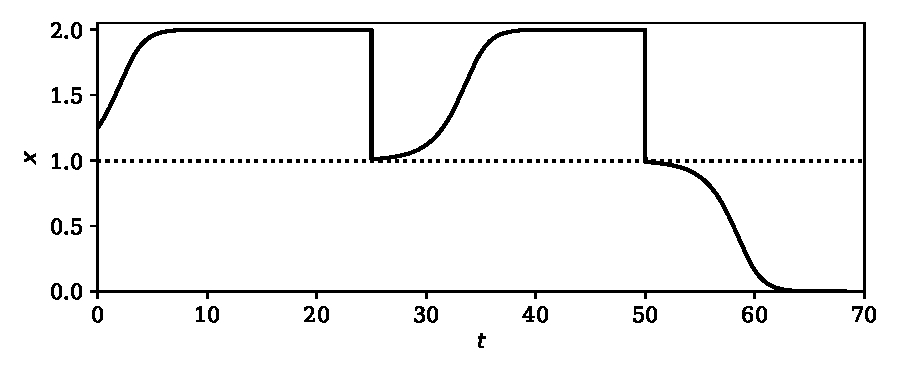
\includegraphics{shock}
  \caption{An example of shock-tipping}
  \label{fig:shock_tipping}
\end{figure}

%Phase tipping?

\section{Early Warning Signals}
Systems behaving 1D. Critical Slowing Down. Use of variance and
autocorrelation. Other methods. Fluctuation dissipation theorem.
Resilience. Critical Speeding up. Hasselmann. Loreenz. Leith. 
Why is it hard to model?
\section{Non-autonomous Topics}
Overshoot. Timescales. Slow fast systems.